\section{In-Network Memory Management}
\label{sec:mindintro}
Data center network bandwidth is rapidly approaching and may soon surpass intra-server resource interconnect speeds~\cite{terabitethernet, remotememory}, sparking increased interest in memory disaggregation from both academia~\cite{memdisagg2, memdisagg3, memdisagg4, memdisagg5, memdisagg6, memdisagg1, legoos, infiniswap, fastswap, disagg, disaggfault} and industry~\cite{industry0, industry1, industry2, industry3, industry4, industry5}. By separating compute and memory into network-attached resource blades, memory disaggregation improves resource utilization, hardware heterogeneity, elasticity, and failure handling in data centers.

However, memory disaggregation faces three major challenges. First, remote memory access must have low latency and high throughput, with targets of $10~\mu$s latency and 100 Gbps bandwidth per compute blade~\cite{legoos, infiniswap, fastswap, disagg}. Second, both compute and memory resources need to scale elastically. Finally, adoption requires support for unmodified applications.

Despite extensive research, no solution fully addresses all three challenges. Many approaches demand application modifications due to hardware~\cite{industry1, industry2, nwsupport, memdisagg4}, programming model~\cite{piccolo, grappa}, or memory interface changes~\cite{farm, ramcloud, herd}. Transparent access systems~\cite{legoos, infiniswap, fastswap} limit compute elasticity by confining processes to a single compute blade to avoid performance degradation from cache coherence traffic.

We introduce \mind, the first memory management system for rack-scale disaggregated memory that meets all three requirements. \mind places the \mmm within the network fabric, treating the network as a CPU-memory interconnect. By using programmable network switches~\cite{progswitch1, progswitch2, progswitch3} as MMUs, \mind enables a high-performance shared memory abstraction with minimal latency and bandwidth overheads through line-rate processing~\cite{progswitch1}.

To meet the three requirements of memory disaggregation, \mind effectively navigates the constraints of programmable switches and leverages their capabilities for in-network memory management by redesigning traditional memory management as follows:
\begin{itemize}
  \item \textbf{Global Virtual Address Space}: \mind employs a globally shared virtual address space, range-partitioned across memory blades, minimizing the number of address translation entries stored in switch ASIC on-chip memory. Additionally, it uses a load-balancing physical memory allocation mechanism to optimize memory throughput across memory blades.
  
  \item \textbf{Domain-Based Memory Protection}: Inspired by capability-based schemes~\cite{capabilityaddr, cap, opal}, \mind decouples memory permissions from address translation entries, enabling fine-grained, flexible protection while reducing on-chip memory overhead on the switch ASIC.
  
  \item \textbf{Cache Coherence via Directory-Based MSI}: \mind adapts directory-based MSI coherence~\cite{msi} to the in-network environment and uses network-centric hardware primitives like switch ASIC multicast to minimize network overhead in its coherence protocol.
  
  \item \textbf{Dynamic Memory Region Sizing}: To address the challenge of limited switch ASIC memory, \mind tracks memory regions at coarse granularity, which can cause performance degradation from false invalidations. \mind mitigates this with a novel sizing algorithm that dynamically adjusts region sizes, balancing storage efficiency and minimizing performance losses due to false invalidations.
\end{itemize}

We realize \mind design on a disaggregated cluster emulated using traditional servers connected by a programmable switch. Our results show that \mind enables transparent resource elasticity for real-world workloads while matching the performance for prior memory disaggregation proposals. 

We also find that while \mind is competitive with compared systems, workloads with high read-write contention experience sub-linear scaling with more threads due to limitations of current hardware. Current x86 architectures preclude realization of relaxed consistency models commonly employed in shared memory systems~\cite{gam}, and the switch TCAM capacity is close to saturated with cache directory entries for such workloads. We discuss approaches that could enable better scaling with future improvements in switch ASIC and compute blade architectures in \S\ref{sec:discussion}.


This section motivates \mind. We discuss key enabling technologies (\S\ref{ssec:assumptions}), followed by challenges in realizing memory disaggregation goals using existing designs (\S\ref{ssec:challenges}).

\paragraphb{Assumptions} We focus on memory disaggregation at the \textit{rack-scale}, where memory and compute blades are connected by a single programmable switch. Similar to prior work~\cite{memdisagg2, memdisagg3, memdisagg4, memdisagg5, memdisagg6, memdisagg1, legoos, disagg}, we restrict our scope to \textit{partial} memory disaggregation: while most of the memory is network-attached, CPU blades possess a small amount (few GBs) of local DRAM as cache.

\begin{figure}[t]
  \centering
  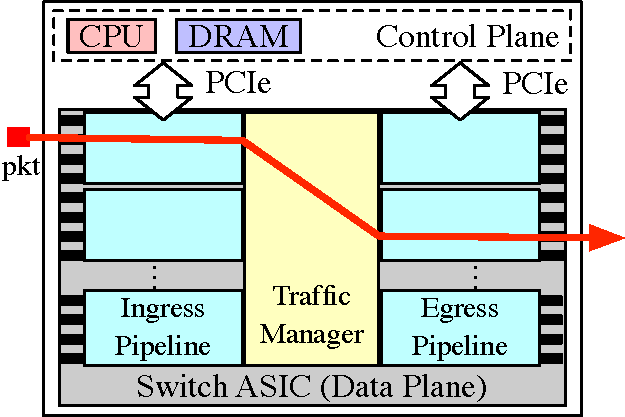
\includegraphics[width=0.44\columnwidth]{fig/mind/prog-switch.pdf}\hfill
  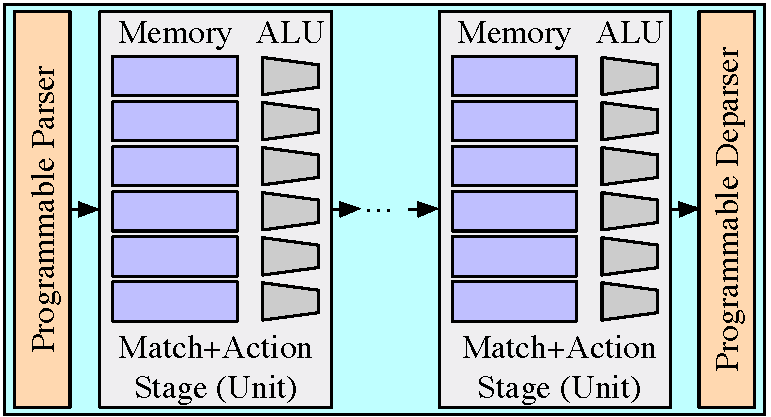
\includegraphics[width=0.54\columnwidth]{fig/mind/prog-pipeline.pdf}
  \vspace{-0.7em}
  \caption[Enabling technologies for \mind]{\textbf{Enabling technologies for \mind.} (left) Programmable switch architecture and (right) Switch ingress/egress pipeline.}
  \vspace{-0.5em}
  \label{fig:trad-directory}
  \label{fig:prog-pipeline}
  \label{fig:background}
\end{figure}

\begin{table*}
  \caption[In-network technology tradeoffs]{\textbf{In-network technology tradeoffs.}}\vspace{-1em}
  \label{fig:switchtradeoff}
  \scriptsize
    \renewcommand{\arraystretch}{1.2}
    \begin{tabular}{c|c|c|c|c}
      \hline
      & RMT & FPGA & Custom ASIC & CPU \\\hline\hline
      Line-rate & \cmark & \cmark & \cmark & \xmark \\
      Available & \cmark & \cmark & \xmark & \cmark \ \\
      Low Power & \cmark & \xmark & \cmark & \xmark\\
      Low Cost & \cmark & \xmark & \cmark & \xmark\\
      \hline
    \end{tabular}
  \end{table*}

We now briefly describe \mind's enabling technologies.

\paragraphb{Programmable switches} In recent years, programmable switches have evolved along two well-coordinated directions: development of P4~\cite{p4, p4paper, dcp4}, a flexible programming language for network switches, and design of switch hardware that can be programmed with it~\cite{rmt, progswitch2, progswitch3, progswitch4}. These switches host an application-specific integrated circuit (ASIC), along with a general purpose CPU with DRAM, as shown in Figure~\ref{fig:background}~(left). The switch ASIC comprises ingress pipelines, a traffic manager and egress pipelines, which process packets in that order. Programmability via P4 is facilitated through a programmable parser and match-action units in the ingress/egress pipelines, as shown in Figure~\ref{fig:prog-pipeline}~(right). Specifically, the program defines how the parser parses packet headers to extract a set of fields, and multiple stages of match-action units (each with limited TCAM/SRAM and ALUs) process them. The general purpose CPU is connected to the switch ASIC via a PCIe interface, and serves two functions: (i) performing packet processing that cannot be performed in the ASIC due to resource constraints, and, (ii) hosting controller functions that compute network-wide policies and push them to the switch ASIC.

While the above focuses on switch ASICs with Reconfigurable Match Action Tables (RMTs)~\cite{rmt}, it is possible to realize \mind using FPGAs, custom ASICs, or even general purpose CPUs. While each of them exposes different tradeoffs (Table~\ref{fig:switchtradeoff}), we adopt RMT switches due to their performance, availability, power and cost efficiency.

\paragraphb{DSM Designs} Traditionally, shared memory has been explored in the context of NUMA~\cite{sgiorigin, amdopteron1, amdopteron2, intelqpi1, intelqpi2} and distributed shared memory (DSM) architectures~\cite{munin, midway, dpram, gam, dash}. In such designs, the virtual address space is partitioned across the various nodes, \ie, each partition has a \textit{home} node that manages its metadata, \eg, the page table. Each node also additionally has a cache to facilitate performance for frequently accessed memory blocks. We distinguish memory blocks from pages since caching granularities, \ie, block, can be different from memory access granularities, \ie, page. 

With the copies of blocks potentially residing across multiple node caches, coherence protocols~\cite{msi, mesi, mesif, moesi, mosi} are required to ensure each node operates on the latest version of a block. In popular directory-based invalidation protocols like MSI~\cite{msi} (used in \mind), each memory block can be in one of three states: \textbf{M}odified (\textbf{M}), where a single node has exclusive read and write access to (or, ``owns'') the block, \textbf{S}hared (\textbf{S}), where one or more caches have shared read-only access to the block, and \textbf{I}nvalid (\textbf{I}), where the block is not present in any cache. A directory tracks the state of each block, along with the list of nodes (``sharer list'') that currently hold the block in their cache. The directory is typically partitioned across the various nodes, with each home node tracking directory entries for its own address space partition. Memory access for a block that is not local involves contacting the home node for the block; it triggers a state transition and potential invalidation of the block across other nodes, followed by retrieving the block from the node that owns the block. While it is possible to realize more sophisticated coherence protocols, we restrict our focus to MSI in this work due to its simplicity --- we defer a discussion of other protocols to \S\ref{sec:discussion}.

Extending the benefits of resource disaggregation to memory and making them widely applicable to cloud services demands (i) low-latency and high-throughput access to memory, (ii) a transparent memory abstraction that supports elastic scaling of memory \textit{and} compute resources without requiring modifications to existing applications. Unfortunately, prior designs for memory disaggregation expose a hard tradeoff between the two goals. Specifically, transparent elastic scaling of an application's compute resources necessitates a shared memory abstraction over the disaggregated memory pool, which imposes non-trivial performance overheads due to the cache-coherence required for both application data \textit{and} memory management metadata. We now discuss why this tradeoff is fundamental to existing designs. We focus on page-based memory disaggregation designs here, and defer the discussion of other related work to \S\ref{sec:related}.

\begin{table}
    \caption[Parallels between memory \& networking primitives]{\small \textbf{Parallels between memory \& networking primitives.}}\vspace{-1em}
    \label{table:isomorph}
    \centering
    \scriptsize
    \renewcommand{\arraystretch}{1.2}
    \begin{tabular}{p{2cm} p{0.7cm}p{2cm}}
      \hline
      \textbf{Virtual Memory} &$\Longleftrightarrow$ &\textbf{Networking} \\\hline\hline
      Memory allocation&&IP assignment\\
      Address translation &&IP forwarding\\
      Memory protection  &&Access control\\
      Cache invalidations &&Multicast\\
      \hline
    \end{tabular}
    \vspace{-1em}
\end{table}

\subsection{\mind Overview}
\label{ssec:mindoverview}

\begin{figure*}[!t]
\centering
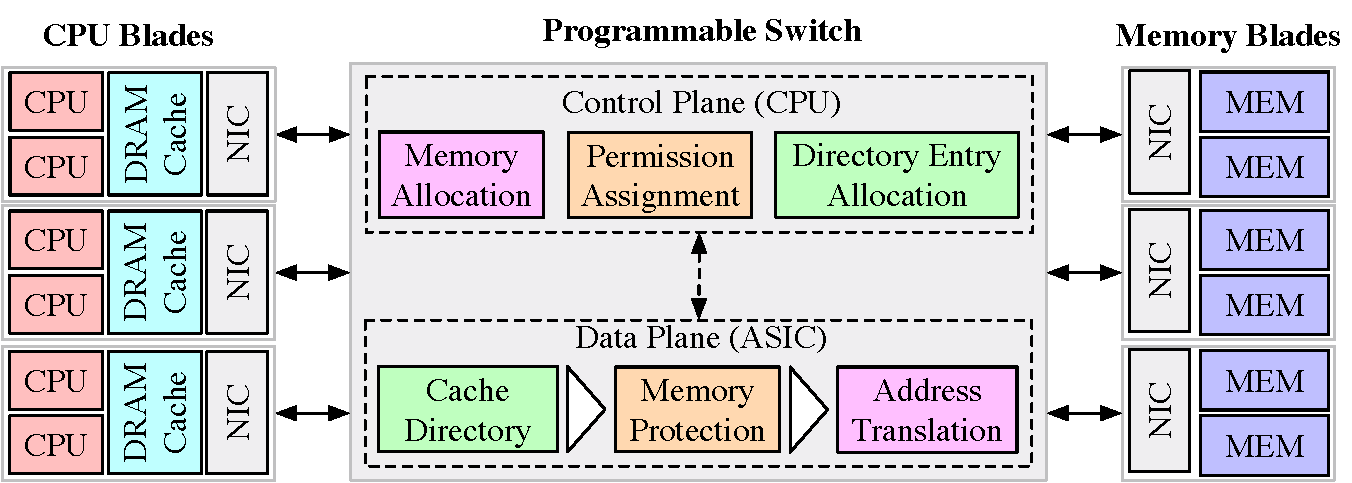
\includegraphics[width=0.55\textwidth]{fig/mind/design}\hspace{3em}
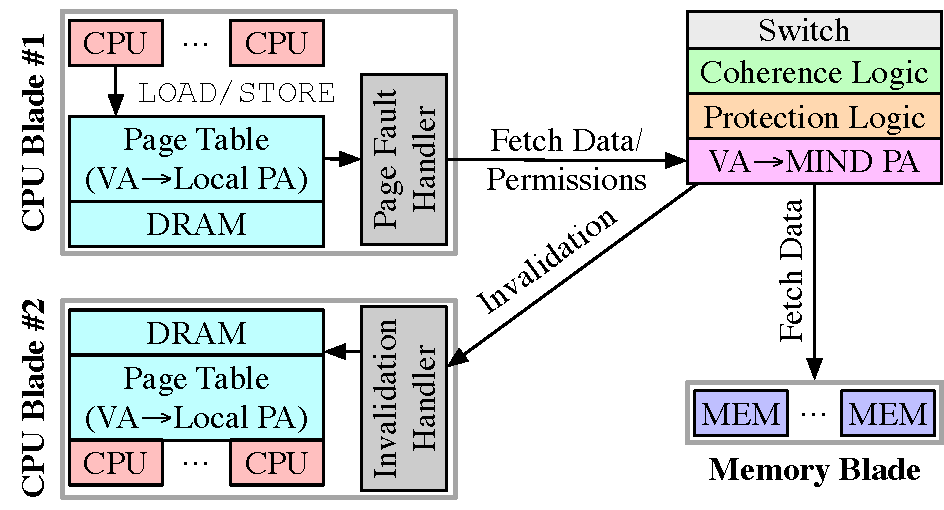
\includegraphics[width=0.35\textwidth]{fig/mind/data_flow}%\vspace{-1em}
\vspace{-0.5em}
\caption[High-level \mind architecture and data flow for memory accesses in \mind]{\textbf{(left) High-level \mind architecture, and, (right) data flow for memory accesses in \mind.} See \S\ref{ssec:design} for details.}
\label{fig:system_diagram}
\end{figure*}

To break the tradeoff highlighted above, we place memory management \textit{in the network fabric} for three reasons.
First, the network fabric enjoys a central location in the disaggregated architecture. Therefore, placing memory management in the data access path between compute and memory resources obviates the need for metadata coherence. 
Second, modern network switches~\cite{progswitch1, progswitch2, progswitch3} permit the implementation of such logic in integrated programmable ASICs. We show that these ASICs are capable of executing it at line rate even for multi-terabit traffic. In fact, many memory management functionalities have similar counterparts in networking (\autoref{table:isomorph}), allowing us to leverage decades of innovation in network hardware and protocol design for disaggregated memory management.
Finally, placing the cache coherence logic and directory in the network switch permits the design of specialized in-network coherence protocols with reduced network latency and bandwidth overheads, as we show in \S\ref{sec:design}. 

Effective in-network memory management requires: (\text{i}) \emph{efficient storage}, by  minimizing in-network metadata given the limited memory on the switch data plane;  (\textit{ii}) \emph{high memory throughput}, by load-balancing memory traffic across memory blades; (\textit{iii}) \emph{low access latency to shared memory}, via efficient cache coherence design that hides the network latency.


\subsubsection{Design Overview}
\label{sssec:design}

\mind exposes a \textit{transparent virtual memory} abstraction to applications, similar to server-based OSes. Unlike prior disaggregated memory designs, \mind places all \mmm in the network, instead of CPU or memory blades~\cite{infiniswap, fastswap}, or a separate global controller~\cite{legoos}. 

Figure~\ref{fig:system_diagram}~(left) provides an overview of \mind design, while Figure~\ref{fig:system_diagram}~(right) depicts the data flow for memory accesses in \mind. The \textit{CPU blades} run user processes and threads, and possess a small amount of local DRAM that is used as a cache. All memory allocations (\eg, via \texttt{mmap} or \texttt{sbrk}) and deallocations (\eg, via \texttt{munmap}) from the user processes are intercepted at the CPU blade, and forwarded to the \textit{switch control plane}. The control plane possesses a global view of the system, which it leverages to perform memory allocations, permission assignments, \etc, using principle \textbf{P2}, and respond to the user process. All memory \code{LOAD}/\code{STORE} operations from the user processes are handled by the CPU blade cache (\S\ref{ssec:caching}). The cache is virtually addressed\footnote{Note that while it is hidden from applications, CPU blades maintain a local page-based virtual memory abstraction to translate \mind virtual addresses to physical addresses for cached pages in local DRAM (Figure~\ref{fig:system_diagram}~(right)).}, and stores permissions for cached pages to enforce memory protection. If a page is not locally cached, the CPU blade triggers a page-fault and fetches the page from \textit{memory blades} using RDMA requests, evicting other cached pages if necessary. Similarly, if the memory access requires an update to a cached block's coherence state (\eg, \code{STORE} on a Shared or \textbf{S} block), a page-fault is triggered to initiate cache coherence logic at the switch. Note that the page-fault based design requires \mind to perform page-level remote accesses, although future CPU architectures may enable more flexible access granularities (\S\ref{sec:discussion}).

Since the CPU blade does not store memory management metadata, the RDMA requests are for virtual addresses and do not contain endpoint information (\eg, IP address) for the memory blade that holds the page. Consequently, the \textit{switch data plane} intercepts these requests. It then performs necessary cache coherence logic, including lookups/updates to the cache directory and cache invalidations on other CPU blades (\S\ref{ssec:caching}, \S\ref{sec:algorithm}). In parallel, the data plane also ensures the requesting process has permissions to access the requested page (\S\ref{subsec:mem_prot}). If no CPU blade cache holds the page, the data plane translates the virtual addresses to physical addresses (\S\ref{subsec:addr_trans}), forwarding the request to the appropriate memory blade. These memory management functionalities are decoupled as separate modules following \textbf{P1}, and efficiently realized in the switch ASIC following \textbf{P3}.

In \mind's design, the memory blades simply store the actual memory pages, and serve RDMA requests for physical pages. Unlike prior works that employ RPC handlers and polling threads~\cite{legoos}, \mind leverages one-sided RDMA operations~\cite{farm} to obviate the need for any CPU cycles on the disaggregated memory blades. This is a step towards true hardware resource disaggregation, where memory blades need no longer be equipped with any general-purpose CPUs.

\subsection{\mind Design}
\label{ssec:minddesign}

Placing memory management logic and metadata in the network provides the opportunity for simultaneously achieving memory performance and resource elasticity. We now describe how \mind optimizes for the individual goals of memory allocation and addressing (\S\ref{subsec:addr_trans}), memory protection (\S\ref{subsec:mem_prot}), and cache coherence (\S\ref{ssec:caching}), while operating under the constraints of programmable switches. Finally, we detail how \mind handles failures (\S\ref{subsec:acking}). %We now describe how \mind achieves the same.

\subsubsection{Memory Allocation \& Addressing}
\label{sssec:addr_trans}

Traditional virtual memory uses fixed sized pages as the basic units for both translation and protection; as a result, it cannot achieve the goal of storage efficiency without increasing memory fragmentation: small pages reduce memory fragmentation but require more translation entries, and vice versa.  Following \textbf{P1}, \mind overcomes this by \textit{decoupling} address translation and protection.  That is, \mind's translation is blade-based while protection is \code{vma} based (\S\ref{subsec:mem_prot}).

\paragraphb{Storage-efficient address translation} \mind eschews page-based protection but uses a \textit{single global virtual address-space} across all processes, allowing translation entries to be shared across them. Our approach builds on decades of research on virtual memory designs that also exploit a single address space~\cite{cheri, cap, gam, grappa, opal}, but adds techniques to minimize storage overheads for in-network address translation.
In particular, \mind \textit{range partitions} the virtual address space across different memory blades, such that the entire virtual-address space maps to a contiguous range of physical address space. This allows us to use a single translation entry for each memory blade: any virtual address that falls within its range can be directly routed to that memory blade, minimizing the storage required on switch data plane. In \mind, this mapping only changes when new memory blades join, old ones retire or if memory is moved between blades.

\paragraphb{Balanced memory allocation \& reduced fragmentation} \mind's control plane, leveraging its global view of allocations (\textbf{P2}), tracks the total amount of memory allocated on each memory blade and places a new allocation on the blade with the least allocation, to achieve near-optimal load-balancing. We validate this empirically in \S\ref{sec:evaluation}.

Moreover, since there is a one-to-one mapping between virtual and physical addresses within a particular memory blade, \mind minimizes external fragmentation at each memory blade by using traditional virtual memory allocation schemes that have evolved to facilitate the same, \eg, first-fit allocator in our implementation~\cite{firstfit}.
The result of memory allocation is a virtual memory area (\texttt{vma}), identified by the base virtual address and length of the area, \eg, 
  {{\small <\texttt{0x00007f84b862d33b}, \texttt{0x400}>}}
for a $1$KB area. 
As will be elaborated in \S\ref{subsec:mem_prot}, \code{vma} is the basic unit of protection in \mind.
This allows multiple processes to have non-overlapping \code{vma}s on the same blade, minimizing memory fragmentation.
 
\paragraphb{Isolation} We note that \mindx's global virtual address-space does not compromise on \textit{isolation} between processes. First, since the switch intercepts allocation requests across all compute blades, and possesses a global view of valid allocations at any time, it can easily ensure allocations are non-overlapping across different processes. Second, we show in \S\ref{subsec:mem_prot} that \mind's \code{vma}-based protection allows flexible access control between processes in a single global virtual address-space.

\paragraphb{Transparency via outlier entries} \mindx's one-to-one mapping between virtual and physical addresses does not preclude supporting unmodified applications with static virtual addresses embedded within their binaries, or OS optimizations such as page migration~\cite{pagemigrations}, \ie, moving pages from one memory blade to another. \mind maintains separate \textit{range-based} address translations~\cite{rangetranslations} for physical memory regions that correspond to static virtual addresses or migrated memory. These \textit{outlier} entries are stored succinctly in the switch TCAM, where the TCAM's longest-prefix matching (LPM) property ensures that only the most specific entry (\ie, one with the longest prefix) is considered when translating a virtual address, ensuring correctness.

\subsubsection{Memory Protection}
\label{sssec:mem_prot}

As \mind decouples translation and protection, it uses a separate table to store memory protection entries in the data plane. 
Consequently, an application can assign access permissions to a \code{vma} of any size.
The size of this protection table is proportional to the number of \code{vma}s. We find this number is reasonably small in our experiments and the protection table can easily fit in the switch ASIC even for a wide range of memory-intensive applications (\S\ref{sec:evaluation}). This is because the first-fit allocator and Linux's \code{glibc} allocation requests~\cite{glibc-alloc} do a good job of ensuring \code{vma}s are large and contiguous. 

\paragraphb{Fine-grained, flexible memory protection} Similar to prior work on capability-based systems~\cite{cheri, capabilityaddr}, \mind supports two key abstractions: \textit{protection domains} and \textit{permission classes}. Protection domains identify the entity that may (or may not) have permissions to access a particular memory region of arbitrary size, while the permission class identifies what the entity can do to the memory region. 
\mind's control plane exposes a set of APIs for memory allocation and permission changes that allows an application to specify a protection domain identifier (\code{PDID}) for an arbitrary virtual memory area (\code{vma}) and assign a permission class (\code{PC}) to the pair \code{<PDID}, \code{vma>}. 
The mapping \code{<PDID}, \code{vma>} $\rightarrow$ \code{PC} is stored as an entry in the protection table in the data plane. For existing applications, \mind simply takes the process identifier (\code{PID}) as the \code{PDID},  and uses Linux memory permissions (\eg, read-only, read-write, \etc) as permission classes. Note that \mind \textit{can} support richer memory protection semantics than traditional OSes, \eg, user programs that serve multiple client sessions, such as ssh servers or database services, can assign a separate protection domain per session to prevent one session from accessing data from other sessions~\cite{cheri}. 

Following principle \textbf{P3}, we leverage TCAM-based parallel range matches in the programmable switch ASIC --- typically used for IP subnet matches --- to efficiently support fine-grained matching for \code{<PDID}, \code{vma>} entries embedded in memory access requests and obtain corresponding the permission class (\code{PC}). If there is a mismatch between \code{PC} and the memory access type, or the \code{<PDID}, \code{vma>} entry does not exist, the request is rejected.

\paragraphb{Optimizing for TCAM storage} One limitation of TCAM is that each of its entries can only match power-of-two ranges. \mind overcomes this by splitting an arbitrary-sized virtual address range into multiple power-of-two-sized entries. Note that the number of entries required for a range of size $s$ is upper-bounded by $\lceil\log_2(s)\rceil$. In order to meet our goal of storage efficiency in the switch data plane, the control plane (1) only performs virtual address allocations that are aligned with the power-of-two sizes to ensure each region can be represented using a single TCAM entry, and (2) coalesces adjacent entries with if they belong to the same protection domain and have the same permission class. Interestingly, memory allocations requested by underlying libraries (\eg, \texttt{glibc}) are mostly in power-of-two sizes anyway, enabling storage-efficiency for TCAM entries.

\subsubsection{Caching \& Cache Coherence}
\label{sssec:caching}

In \mind design, while the caches\footnote{Note that we use the term `cache' to refer to the DRAM at the CPU blade under the partial disaggregation model, and not hardware (L1/L2/L3) caches.} reside on compute blades, the coherence directory and logic reside in the switch. This already permits access to the cache directory in half a round-trip, significantly reducing the latency overheads for the coherence protocol execution. For MSI protocol, even the most expensive and relatively uncommon transitions (\ie, \textbf{M}$\rightarrow$\textbf{S/M}) incur two round-trips, while common transitions incur only a single round-trip, as we show in \S\ref{ssec:bottlenecks}. While performance is a primary objective in \mind's cache coherence, the coherence protocol must also be realizable under the compute and memory constraints of switch ASICs. We now outline challenges in adapting traditional cache management to our in-network setting, along with how \mind resolves them.

\subsubsection{Storage vs. performance tradeoff}\label{ssec:storagevsperf}\hfill\\
Traditional caching and cache coherence mechanisms applied to \mind expose a tradeoff between cache performance and the storage efficiency at the switch data plane. Specifically, reducing the number of directory entries requires larger cache granularities (\ie, larger memory blocks), which results in worse performance. For instance, when large (\eg, $2$ MB) memory blocks are used, updating a small (\eg, $4$ KB) region within the block will invalidate the entire block. We refer to these invalidations as \emph{false invalidations} --- dirty pages invalidated along with the requested page because there are in the same memory block tracked by a directory entry. This leads to wastage in both memory bandwidth and cache capacity, \ie, fewer frequently accessed data items in the cache. We empirically highlight this tradeoff in \S\ref{ssec:sensitivity}.

\mind addresses this challenge using two approaches: it decouples the cache and directory granularities (following principle \textbf{P1}), and appropriately sizes the memory region tracked by each cache directory entry leveraging the global view of memory traffic at the control plane (following principle \textbf{P2}), as we describe next.

\paragraphb{Decoupling cache access \& directory entry granularities} Our first approach employs principle \textbf{P1} --- decoupling the granularity of cache (and memory) accesses from the granularity at which cache coherence is performed. This allows memory accesses (\eg, evictions or remote memory reads) to be performed at finer granularities, while directory entries are tracked at coarser granularities. Specifically, accesses to the local DRAM cache at CPU blades, and even the movement of data between the CPU caches and memory blades, occur at the fine page granularity ($4$ KB in \mind, similar to prior work~\cite{legoos, infiniswap, fastswap}). However, the coherence protocol tracks directory entries (stored at the switch data plane) at larger, variable-sized \textit{region} granularities --- when a $4$ KB page is cached at a CPU blade, \mind creates a directory entry for the region that contains the page. An invalidation of the region triggers an invalidation of all dirty pages in the region, as tracked by the individual CPU blades that cache them.

\paragraphb{Storage \& performance-efficient sizing of \textit{regions}} Even with the decoupling described above, the region \textit{sizes} still expose a tension between coherence performance (\eg, larger false invalidation counts due to larger region sizes) and directory storage efficiency (\eg, more directory entries due to smaller region sizes). To appropriately size regions, \mind leverages global view of memory traffic at the switch control plane (\textbf{P2}). Briefly, \mind starts each directory entry with a very large memory region; when the overhead due to false invalidation is high, it splits the region and creates a new directory entry. It does so repeatedly, until either the overhead is below a predetermined threshold, or the region size reaches $4$~KB, \ie, the page size. In doing so, \mind dynamically customizes the region sizes to resolve the tension between performance and directory storage efficiency using a novel \sizing algorithm --- we defer its details to \S\ref{sec:algorithm}.

\subsubsection{In-Network Coherence Protocol}\label{subsec:cache_dir}\hfill\\
\noindent
Due to the limited computational capability at the switch ASIC, \mind employs the simple directory-based MSI coherence protocol~\cite{msi}. While we defer the implementation details of the coherence protocol to \S\ref{ssec:switchimpl}, we highlight here how \mind employs network-centric hardware primitives to efficiently realize the coherence protocol in the switch, leveraging principle \textbf{P3}. Specifically, several state transitions in the MSI protocol require generating invalidation requests to CPU blades that have shared access to a region, to ensure correctness. To facilitate this in a network-efficient manner, we leverage \textit{multicast} functionality supported natively in most switches --- we create a multicast group for all CPU blades in the rack, and send an invalidation request containing the list of sharers to the group. However, broadcasting invalidations to blades not in the sharer list would consume unnecessary network bandwidth. As such, we embed the sharer list within the invalidation request, and drop requests in the egress path of the switch data plane if the output port does not lead to a blade in the sharer list.

\subsubsection{Handling Failures}
\label{sssec:acking}

We now discuss how \mind handles failures at different components in our disaggregated architecture.

\paragraphb{CPU, memory blade and switch failures} \mind does not innovate on fault-tolerance for CPU and memory blade failures: mechanisms developed in prior work~\cite{legoos, infiniswap, disaggfault} for fault tolerance can be readily adapted to our design. To handle switch failures, we consistently replicate the control plane at a backup switch --- on a failure, the data plane state is reconstructed at the backup switch using the control plane state. Since the control plane is only updated infrequently due to metadata operations (\eg, system calls), the overhead added due to such replication in minimal.

\paragraphb{Communication failures} \mind uses ACKs and timeouts to detect packet losses. When a memory access triggers invalidations, the requesting compute blade waits for ACKs indicating successful invalidation from all sharers, and resends the request if timeout occurs. If the compute blade does not receive an ACK even after a predefined number of retransmissions, it sends a \code{reset} message for the corresponding virtual address to the switch control plane. This, in turn, forces all compute blades to flush their data for that address and removes the corresponding cache directory entry in the data plane. This \code{reset} mechanism prevents deadlocks when compute blades fail in the middle of a cache coherence state transition.

We show in \S\ref{sec:evaluation} that appropriate epoch sizing allows us to ensure both assumptions for our evaluated workloads.

\subsection{\mind Implementation}
\label{ssec:mindimpl}

We now describe \mind implementation. \mind exposes Linux memory and process management system call APIs, and splits its kernel components across CPU blade and the programmable switch. We now describe these kernel components, along with the RDMA logic required at the memory blade.

\subsubsection{CPU Blade}
\label{sssec:cpumemimpl}

\mind assumes a partial disaggregation model, where the CPU blades possess a small amount of local DRAM as cache (\S\ref{ssec:assumptions}). The CPU blades in our prototype use traditional servers with no hardware modifications. We implemented CPU blade kernel components as a modified Linux kernel 4.15. \mind provides transparent access to the disaggregated memory, by modifying how \code{vma}s and processes are managed and how page faults are handled at the CPU blade, as we detail next.

\paragraphb{Managing \code{vma}s} To handle the creation and removal of \code{vma}s due to process heap allocation/deallocation requests, such as \code{brk}, \code{mmap}, and \code{munmap}, the kernel module intercepts such requests from the process and forwards them to the control plane at the switch over a reliable TCP connection. The switch subsequently creates new \texttt{vma} entries, and responds with the same return value (\eg, virtual address of the allocated \code{vma}) as the local version of the system calls --- ensuring transparency for user applications. The switch returns Linux-compatible error codes (\eg, \code{ENOMEM}) if there are any errors.

\paragraphb{Managing processes} The kernel module also intercepts and forwards process creation and termination requests, such as \code{exec} and \code{exit}, to the switch control plane, which maintains the internal representation of processes (\ie, Linux's \code{task\_struct}) and a mapping between the compute blades and processes they host. \mind assigns threads running on different CPU blades the same PID if they belong to the same process, permitting them to transparently share the same address-space via memory protection and address translation rules installed at the switch. Finally, we do not focus on scheduling in this work and simply place threads and processes across compute blades in a round-robin manner.

\paragraphb{Page fault-driven access to remote memory} When a user application tries to access a memory address not present in the CPU blade cache, a page fault handler is triggered and the CPU blade kernel sends a one-sided RDMA read request to the switch with the virtual address and the requested permission class, i.e., read or write for Linux. At the same time, the page to be used by the user application is registered to the NIC as the receiving buffer, obviating the need for additional data copies. Once the page is received, the local memory structures such as PTEs are populated and the control is returned to the user. Our implementation of the CPU blade DRAM cache is similar to LegoOS~\cite{legoos}, but additionally handles cache invalidations for coherence. Specifically, the cache tracks the set of writable pages locally, and on receiving an invalidation request for a region, it flushes all writable pages in the region and removes all local PTEs.

While the above approach enables transparency for access to disaggregated memory, it presents a significant limitation in our implementation --- it restricts the memory consistency model in \mind to stronger Total Store Order (TSO), and precludes weaker consistency models, \eg, Process Store Order (PSO) used in DSM approaches~\cite{gam}. This is because unlike TSO, PSO enables multiple writes to a cached memory region to be propagated asynchronously, but blocks if there is a subsequent read to the same region. Realizing this relaxation using page faults requires such writes to be buffered at the compute blade's local DRAM cache without triggering a page fault, but triggering one on a subsequent read to the same page. Unfortunately, this is impossible in traditional x86 or ARM architectures, since they do not support triggering a trap on read without also triggering one for a write. Consequently, \mind's stricter TSO model results in limited scalability for workloads with high read/write contention to shared memory regions, as we show in \S\ref{subsec:macro_bench}. We discuss possible architectural changes to address this in \S\ref{sec:discussion}.

\subsubsection{Memory blade} 

Unlike prior disaggregated memory systems~\cite{legoos, infiniswap} or distributed shared memory systems~\cite{gam}, \mind does not require any compute logic or data plane processing logic to run on the memory blades, obviating the need for general purpose CPUs on them. However, since the memory blade in our prototype is realized on traditional Linux servers, we rely on the kernel module at the memory blade to perform RDMA-specific initializations. When a memory blade comes online, its kernel module registers physical memory addresses to the RDMA NIC and reports the mapped address to the global controller. However, subsequent one-sided RDMA requests from CPU blades are handled completely by the memory blade NIC without involving the CPUs. Ideally, memory blades would be realized with all logic, including initialization, completely in hardware, without a CPU. While this would facilitate a memory blade design that is both simple and cheap, it would require new hardware design.

\subsubsection{Programmable Switch}
\label{sssec:switchimpl}

The \mind programmable switch module is implemented on a 32-port EdgeCore Wedge switch with a $6.4$~Tbps Tofino ASIC and an Intel Broadwell processor, $8$~GB RAM and $128$~GB SSD. The general purpose CPU hosts the \mind control program, which performs process, memory and cache directory management. Meanwhile, the ASIC performs address translation (\S\ref{subsec:addr_trans}) and memory protection (\S\ref{subsec:mem_prot}), handles directory state transitions and virtualizes RDMA connections between compute and memory blades. We here provide implementation details of the mechanisms not already described in \S\ref{sec:design}.

\paragraphb{Process \& memory management} The control plane hosts a TCP server to handle system call intercepts from CPU blades, and maintains traditional Linux data structures for process/thread management (\code{task\_struct}) as well as memory management (\code{mm\_struct}, \code{vm\_area\_struct}). On receiving a system call, the control plane modifies the data structures accordingly, and responds with return values consistent with the system calls to ensure transparency.

\paragraphb{Cache directory management} \mind reserves a fixed amount of SRAM at the data plane for storing directory entries, and partitions it into fixed sized slots, one for each \textit{region} entry in \mind. The control plane maintains a \textit{free list} for available slots, and a hash table \textit{used map} which maps the base virtual address for the dynamically sized cache region to the SRAM slot storing its directory entry. All slots are initially added to the free list. \mind creates a directory entry for a region during its allocation by removing an SRAM slot from the free list, populating it with the directory entry with invalid (\textbf{I}) state, creating a match-action rule that maps the block virtual address to the SRAM slot at the data plane, and updating its \textit{used map}. A similar process occurs when a region is split, while removing a directory entry follows the reverse procedure.

\begin{figure}[t]
  \centering
  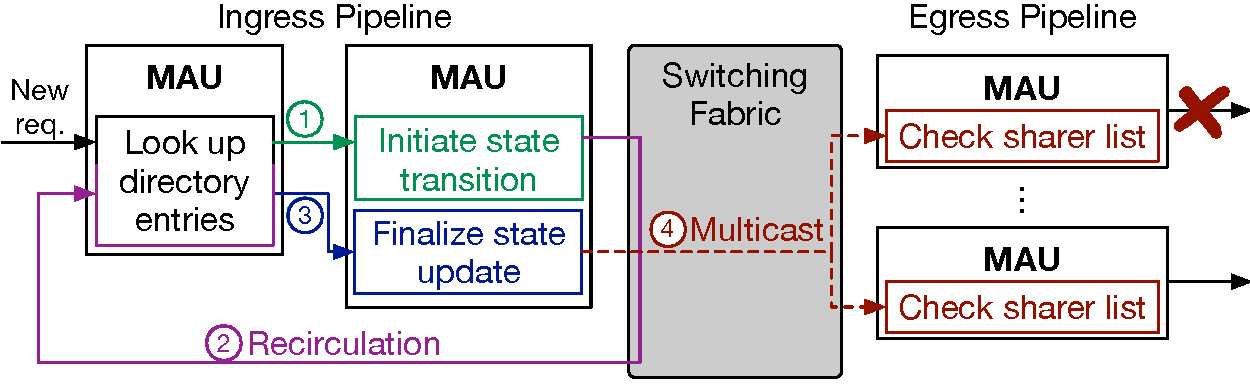
\includegraphics[width=0.97\columnwidth]{fig/mind/cc.pdf}
  \vspace{-0.7em}
  \caption[Performing directory state transitions on switch ASIC]{\textbf{Performing directory state transitions on switch ASIC.}}
  \vspace{-0.5em}
  \label{fig:cc_example}
\end{figure}

\paragraphb{Directory state transitions} We found that a single match-action unit (MAU) in today's switch ASICs is unable to (i) perform a directory entry lookup, (ii) determine the correct translation based on the current block state and memory access request, and (iii) update the directory entry accordingly all at once, due to their limited compute capability. As such, we split the logic for (i-ii) across two MAUs (\circled{1} in Figure~\ref{fig:cc_example}): the first MAU stores the directory entries and performs (i), while the second MAU stores a \textit{materialized} state-transition table containing all possible transitions and corresponding actions to be performed for (ii). Note that explicitly storing the state-transition table trades-off data plane memory capacity to overcome the limited compute cycles in an MAU. To perform (iii), the second MAU \textit{recirculates} the memory access request packet within the switch data plane to send it back to the first MAU (\circled{2}), so that it can update the directory entry according to actions determined by the second MAU (\circled{3}). If the state transition requires cache invalidations, the data plane creates invalidation requests leveraging \textit{multicast}, as described in \S\ref{subsec:cache_dir}. Specifically, these requests are only forwarded to the current sharers for the relevant page (\circled{4}).

\paragraphb{Virtualizing RDMA connections} When a compute blade in \mind issues an RDMA request, it does not know the location of the blade where the page resides. Consequently, the switch data plane in \mind \textit{virtualizes} RDMA connections between all possible CPU-memory blade pairs by transparently transforming and redirecting corresponding RDMA requests and responses between them. Specifically, once an RDMA request's destination blade is identified via address translation or cache coherence, the data plane updates the request's packet header fields such as IP/MAC addresses and RDMA-specific parameters, before forwarding it to the blade.

\subsection{Evaluation}
\label{ssec:mindevaluation}

\begin{figure*}[ht!]
  \centering
  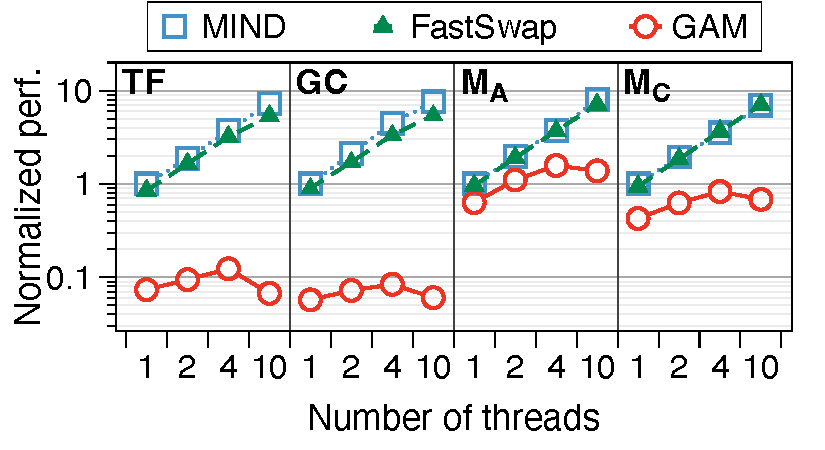
\includegraphics[width=0.345\textwidth]{fig/mind/04_intra}\hspace{-0.25em}
  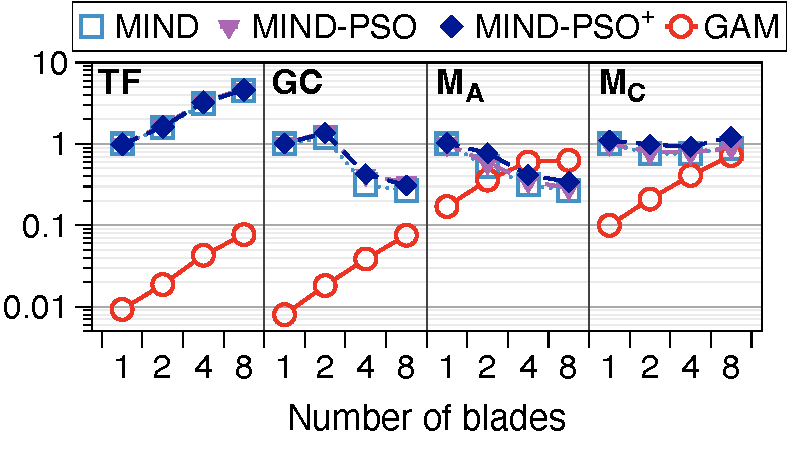
\includegraphics[width=0.3266\textwidth]{fig/mind/04_inter}\hspace{-0.25em}
  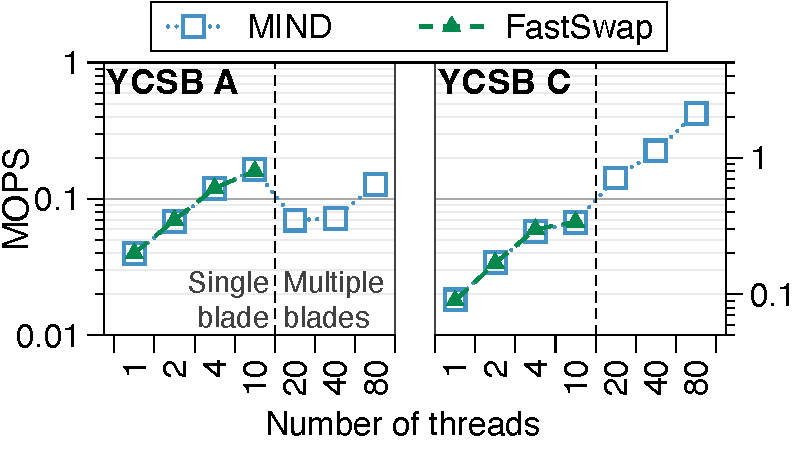
\includegraphics[width=0.3247\textwidth]{fig/mind/04_kvs}
  \vspace{-0.7em}
  \caption[Performance scaling]{\textbf{Performance scaling} (left) on a single compute blade, (center) across compute blades, and (right) for Native-KVS. For (center), each blade runs 10 threads. Performance is normalized by \mind's performance at 1 thread for (left) and 1 blade for (center); the runtimes in seconds for TF, GC, M$_A$ and M$_C$ workloads are 62.8, 59.3, 301.4 and 268.2 for 1 thread, and 69.2, 62.8, 302.3 and 306.9 for 1 blade, respectively.}
\label{fig:perf}
\label{fig:perf_intra}
\label{fig:perf_inter}
\label{fig:perf_kvs}
\end{figure*}


We evaluate \mind to answer the following questions:
\begin{itemize}[topsep=2pt, partopsep=0pt, itemsep=0pt, leftmargin=*]
  \item Can \mind enable transparent elasticity over performant disaggregated memory for real-world workloads?
  \item What are \mind's performance/resource bottlenecks?
\end{itemize}
\paragraphb{Compared systems} We compare \mind against two extreme designs in disaggregated memory: a \textit{transparent} DSM-based approach with cache-coherence that supports compute elasticity, and a \textit{non-transparent} approach that limits compute elasticity to a single compute blade. For the former, we adapt GAM~\cite{gam}, a software-based DSM, to our disaggregated setting where cache directory is implemented at the compute blades. For the latter, we employ FastSwap~\cite{fastswap}, a state-of-the-art swap-based disaggregated memory system. All systems employ RDMA for efficient remote memory accesses. Finally, \mind uses an initial region size of $16$~kB and epoch size of $100$~ms for its \mindalgo algorithm.

\paragraphb{Cluster setup} We used a cluster comprising five servers connected via the programmable switch described in \S\ref{ssec:switchimpl}. We used a single server equipped with two 18-core Intel Xeon processors, $384$~GB of memory and four Nvidia/Mellanox CX-5 $100$~Gbps NICs, to host multiple memory blade VMs. To highlight the overhead and scalability of in-network cache coherence protocol, we used the remaining four machines, each equipped two 12-core Intel Xeon processors and two Nvidia/Mellanox CX-5 $100$~Gbps NICs, to host two CPU blade VMs on each server. Similar to prior work~\cite{legoos}, we emulate the partial disaggregation model by limiting the local DRAM usage at each compute blade to $512$~MB, which is about $25\%$ of the memory footprint for our evaluated workloads. Note that each CPU and memory blade VM in our setup had dedicated access to a separate $100$~Gbps NIC to ensure they represent separate network attached entities.

\paragraphb{Applications and workloads} We use several real-world workloads in our evaluation: TensorFlow~\cite{tensorflow} with ResNet-50~\cite{resnet} on CIFAR-10~\cite{cifar10} (denoted as TF), GraphChi~\cite{graphchi} with PageRank~\cite{pagerank} on Twitter graph~\cite{twitter_graph} (denoted as GC), and Memcached~\cite{memcached} with YCSB~\cite{ycsb_workload} workload A ($50\%$ read, $50\%$ write split, denoted as M$_A$) and workload C ($100\%$ reads, denoted as M$_C$). Since GAM is a \textit{software} DSM system, it requires applications to use a specialized memory API, while \mind and FastSwap are transparent to applications. To ensure consistent comparison under different interfaces, we captured the memory accesses from our workloads using Intel's PIN~\cite{intel_pin}, and used a memory access emulator to generate the exactly same memory accesses across all three systems. In addition, we also present results for native execution of a simple key-value store (denoted as Native-KVS) on \mind and FastSwap, since they support a transparent memory interface.

\subsubsection{Performance Scaling for Real-World Workloads}
\label{sssec:macro_bench}

We start by evaluating \mind's performance scalability.

\paragraphb{Intra-blade scaling} Figure~\ref{fig:perf_intra}~(left) shows performance scaling across all systems as the number of threads is increased on a single compute blade. We report performance as the inverse of runtime, normalized by the performance of \mind for 1 thread. \mind and FastSwap scale almost linearly with more compute blades because of their efficient page-fault driven remote memory accesses. In contrast, GAM scales linearly only up to 4 threads, and sub-linearly after that due to software overheads from its user-level library. For instance, GAM must check access permissions for every memory access by acquiring a lock, while \mind and FastSwap can leverage the hardware MMU to facilitate the same. Such overheads become significant as the compute resources on a single compute blade come under contention at $10$ threads running on a $12$-core node. 

\paragraphb{Inter-blade scaling} Next, we evaluate inter-blade scalability by running $10$ execution threads per-blade, for up to $8$ compute blades. Figure~\ref{fig:perf_inter}~(center) shows our results; here, while \mind's default memory consistency model is strict (TSO, \S\ref{sec:impl}), \mind-PSO denotes the \textit{simulated} performance of \mind with the weaker PSO model (same as GAM). \mind-PSO$+$ additionally simulates the effect of infinite switch capacity for directory storage. Since we are forced to simulate \mind-PSO and \mind-PSO$+$ using traces collected on a real TSO-based system, the traces retain additional TSO-associated queuing delays that we cannot elide, \ie, while our simulations can reorder writes and non-conflicting reads, queuing delays remain; in other words, our \mind-PSO and \mind-PSO$+$ results are underestimates to potential performance of a hardware-based solution. Finally, we omit FastSwap as it does not transparently scale beyond a single compute blade, similar to other disaggregation proposals~\cite{legoos, infiniswap}.

For a machine learning workload (TF), \mind's performance scales well despite its stricter memory consistency model compared to GAM --- doubling the number of compute blades improves \mind's performance by ${\sim} 1.67\times$, with a $59 \times$ speeded compared to GAM at $8$ compute blades. For GC, \mind's performance increases from $1$ to $2$ compute blades, but starts to decrease beyond that. This is because GC's graph traversals incur random and often contentious access to shared data compared to machine learning workloads in TF. GC writes ${\sim} 2.5\times$ more data in shared pages than TF, generating significantly more state transitions to modified (\textbf{M}) state, and incurring frequent invalidations (\S\ref{ssec:bottlenecks}). PSO partly alleviates this overhead by permitting writes to be performed asynchronously, but still does not permit linear scaling beyond $2$ compute blades. Instead, GAM scales better because the performance differential between its local and remote accesses is small --- local accesses are $10\times$ slower than that of MIND (due to software implementation of local accesses), while remote access latencies are similar for both. Consequently, performing more remote accesses (during invalidations) does not impact GAM performance as much as it does for \mind.

Finally, M$_A$ and M$_C$ have more sharers with much larger number of shared writes compared to TF and GC. As a result, \mind does not scale well beyond $1$ compute blade because: (1) more blades contend for acquiring write permission to the same region incurring multiple invalidations and significantly smaller number of local memory accesses, and (2) the directory storage at the switch becomes a bottleneck (as we show in \S\ref{ssec:bottlenecks}), frequently resulting in false invalidations for heavily shared memory regions. We confirm these insights through \mind-PSO and \mind-PSO$+$ simulated results, which show that employing weaker memory consistency models and infinite directory capacity improves \mind's performance to some extent. Note that for M$_C$, \mind's performance increases from $4$ to $8$ blades since the number of invalidations do not increase by much. GAM scales better due to its weaker consistency model, and by leveraging its software implementation to facilitate several memory access reorderings which are not possible in \mind. Consequently, at $8$ compute blades, GAM and \mind-PSO$+$ achieve roughly similar performance.

\paragraphb{Native KVS} Figure~\ref{fig:perf_kvs}~(right) shows the intra- and inter-blade scaling of Native-KVS on \mind and FastSwap for YCSB-A and C workloads. On a single blade, both \mind and FastSwap observe near linear performance scaling for up to $10$ threads. Since FastSwap does not support sharing state across multiple compute blades, we do not report its performance beyond $10$ threads. Similar to our results for M$_A$, \mind does not scale well beyond a single compute blade for the YCSB-A workload ($50\%$ reads, $50\%$ writes) due to high read-write contentions. For the YCSB-C workload, Native-KVS scales linearly even beyond a single blade since it is a read-only workload, incurring no invalidations. Interestingly, YCSB-A workload on Native-KVS scales better than M$_A$ --- we attribute this to better partitioning of KVS state across compute blades in Native-KVS compared to Memcached.

\subsubsection{\mind's Performance and Resource Bottlenecks}
\label{sssec:bottlenecks}

We study \mind bottlenecks in terms of (i) memory access performance, and (ii) memory resources at the switch.

\begin{figure}[t!]
  \centering
  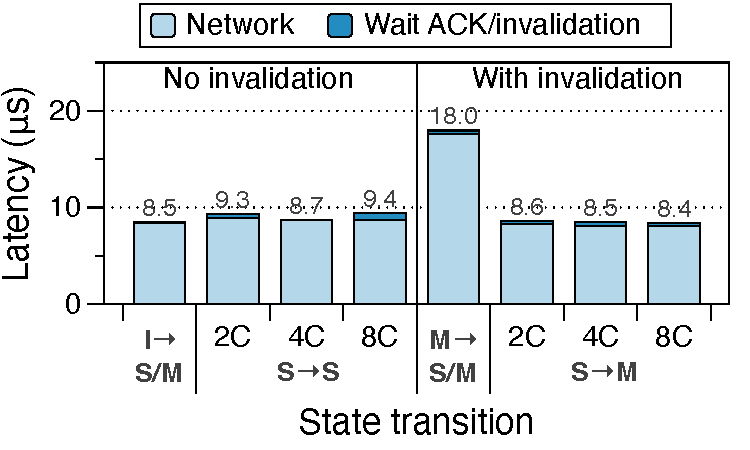
\includegraphics[width=0.58\linewidth]{fig/mind/15_transition_latency}\hfill
  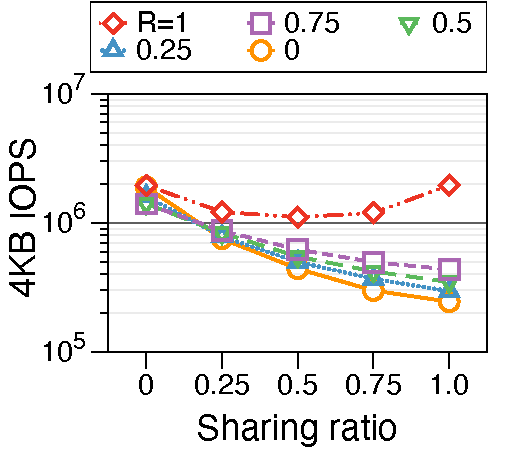
\includegraphics[width=0.40\linewidth]{fig/mind/16_sharing_ratio}
  \vspace{-0.9em}
  \caption[Performance bottlenecks]{\textbf{Performance bottlenecks.} (left) Network latency for state transitions, (right) memory throughput vs. read-write/sharing ratios.}
  \label{fig:micro_latency}
  \label{fig:micro_band} 
  \label{fig:perfbottlenecks}
\end{figure}

\begin{figure*}[ht!]
  \centering
  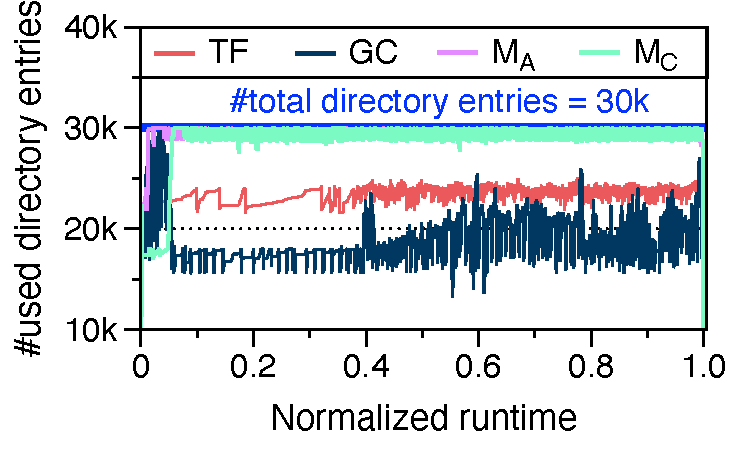
\includegraphics[width=0.3\textwidth]{fig/mind/09_switch_entries_over_time}\hspace{1em}
  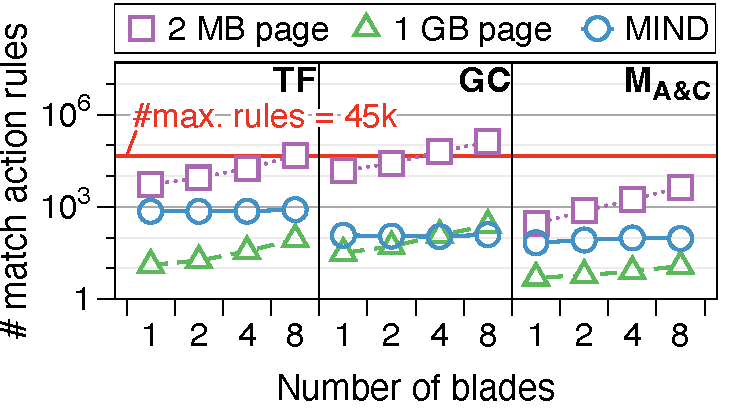
\includegraphics[width=0.31\textwidth]{fig/mind/12_micro_num_entry}\hspace{1em}
  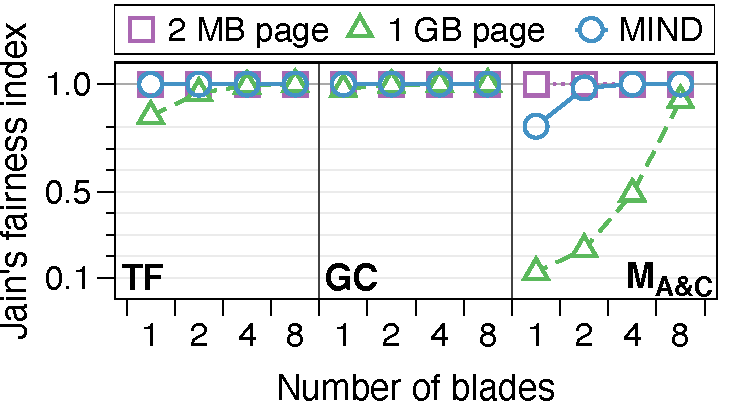
\includegraphics[width=0.31\textwidth]{fig/mind/12_micro_load_balance}
  \vspace{-0.9em}
  \caption[\mind switch resource bottlenecks]{\textbf{\mind switch resource bottlenecks.} (left) Directory entries, (center) match-action entries for heap, (right) load balancing for heap.}
  \label{fig:resbottlenecks}
  \label{fig:micro_load_balance}
  \label{fig:micro_num_entry}
  \label{fig:macro_cache_dir}
\end{figure*}

\begin{figure*}[t!]
  \centering
  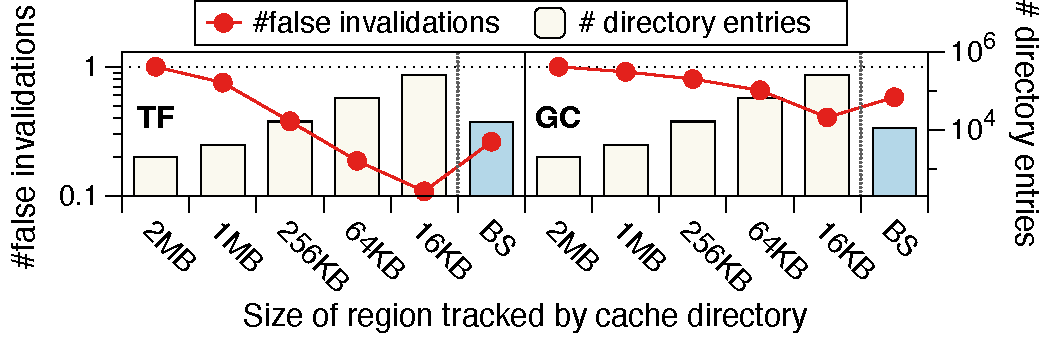
\includegraphics[width=0.49\textwidth]{fig/mind/14d_static_entries}\hspace{2em}
  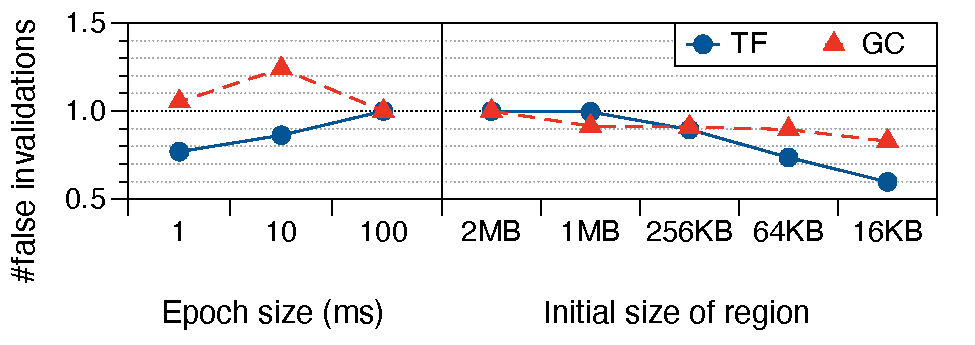
\includegraphics[width=0.46\textwidth]{fig/mind/14c_cache_tradeoff}
  \vspace{-0.9em}
  \caption[Evaluating \mind's \mindalgo algorithm.]{\textbf{Evaluating \mind's \mindalgo algorithm.} (left) Navigating switch storage vs. performance tradeoff. (right) Impact of epoch \& initial region sizing. The number of false invalidations is normalized by value at $2$~MB for region size and $100$~ms for epoch size.}
  \label{fig:storagevperf}
  \label{fig:epoch_size}
  \label{fig:region_size}
\end{figure*}%

\paragraphb{Latency for cache state transitions} Figure~\ref{fig:micro_latency} shows the end-to-end latency due to every possible state transition under the MSI protocol in \mind, including the time required to fetch the data. Note that this figure only shows latency for remote accesses --- local accesses only incur DRAM latency ($<100$~ns). On the x-axis, $2$ -- $8$C indicate the number of CPU blades requesting the same page, and $x \rightarrow y$ denotes the state transition, $x$ and $y$ being the initial and final states. 

When a blade requests read-only (shared, \textbf{S}) mode for a region, and its initial state was either invalid (\textbf{I}) or shared (\textbf{S}), it does not require any invalidations. Consequently, the data fetch can be performed in a single RDMA request (${\sim} 9~\mu$s), as seen in the first four bars. If the transition for a region is either from or to the modified (\textbf{M}) state, the requesting blade must wait until the regions is invalidated at all its previous owners. When transitioning from \textbf{S} to \textbf{M}, the data can be fetched directly from the memory blade via one-sided RDMA operation, while the invalidation at other blades occur in parallel, resulting in a total latency of ${\sim} 9~\mu$s. When the region is initially in \textbf{M} state, the (dirty) data must be fetched from and the region invalidated at the same blade --- its current owner. Therefore, the invalidation and data fetch occur sequentially, resulting in ${\sim} 18~\mu$s latency. Note that since the latency for requests with invalidations is $2\times$ higher than requests without them, a workload's performance depends on the relative proportion of the different types of requests, as we show next.

\paragraphb{Impact of invalidations on memory throughput} Figure~\ref{fig:micro_band}~(right) shows \mind memory throughput across 8 compute blades, running 1 compute thread each, under various read-write and sharing characteristics. We use read ratio to denote the fraction of reads in the workload (remaining accesses are writes), and sharing ratio to denote the portion of memory accesses that occur to a shared region (shared by all threads). We used a total working set size of $400~k$ pages, with the access pattern across them being uniform random. If most accesses are reads, then compute blades can share the same region without triggering invalidations (\textbf{S}$\rightarrow$\textbf{S} in Figure~\ref{fig:micro_latency}). As such, at read-ratio $1$, most of the pages are accessed locally from the cache, resulting in very high memory throughput ($1$-$2\times 10^{6}$ IOPS) for all sharing ratios. Again, at sharing ratio $0$, memory throughput remains high, since accessed pages can remain cached at the compute blade without being invalidated, \ie, most accesses are local. If both the write proportion and sharing ratio are increased, memory throughput drops (by ${\sim} 10\times$ at sharing-ratio $1$), since they trigger a large number number of \textbf{M}$\rightarrow$\textbf{S}, \textbf{S}$\rightarrow$\textbf{M} transitions with invalidations and permit few pages to be accessed locally.

\paragraphb{Cache directory storage} Figure~\ref{fig:macro_cache_dir}~(left) shows the number of cache directory entries stored in the switch data plane in \mind over time for the workloads evaluated in \S\ref{subsec:macro_bench} across 8 compute blades, running 10 threads each. In \mind, we fix the total amount of storage allocated to directory storage to $30$~k entries. For the TF and GC workloads, \mind's \mindalgo algorithm ensures that the number of directory entries remains well below the limit over time. However, the MC$_{A}$ and MC$_{B}$ workloads have a significantly larger number of shared memory regions, with frequent read and write accesses to them; as a consequence, the number of directory entries for the workloads always remains close to the $30$~k limit. Recall from \S\ref{subsec:macro_bench} that one of the key reasons for poor scalability of these workloads is the number of false invalidations triggered due to the relatively coarse granularity of tracking directory entries --- we believe with future switch ASICs likely to be equipped with more TCAM/SRAM, this bottleneck would no longer exist, permitting more efficient scaling under \mind.

\paragraphb{Address translation \& memory protection storage} We study the switch storage overheads due to address translation and memory protection on a setup with 8 memory blades, running the TF, GC, and M$_{A/C}$ workloads; we group $M_A$ and $M_C$ since they have the same memory allocations. Figure~\ref{fig:micro_num_entry}~(center) shows that the number of match action rules due to address translation and memory protection in \mind is almost constant, even as the workload size increases. This is due to \mind's per-memory blade partitioning of the address space, and \code{vma} granularity tracking of memory protection entries. While we have only shown results for three different applications, we find that the number of \code{vma} entries for typical datacenter applications falls in similar ranges, and well under $1$--$2$~k~\cite{vma1, vma2}. In contrast, the number of match-action rules increases linearly with the dataset size for page-based approaches, despite smaller absolute overheads with $1$~GB huge pages. Note that the upper-limit for match-action rules that the switch can store is about $45$~k --- higher than the $30$~k limit for directory entries due to a more compact representation.

\mind's memory allocation also ensures balanced placement of load across memory blades (\S\ref{subsec:addr_trans}), as shown via Jain's fairness index metric~\cite{jain} in Figure~\ref{fig:micro_load_balance}~(right). While $2$~MB pages can achieve similar load-balancing, they do so at the cost of much larger number of address translation entries. $1$~GB pages, on the other hand, observes poor load balancing for allocation-intensive workloads (M$_{A/C}$).



\subsection{Summary}

We now discuss the limitations of the current \mind implementation and future research directions to address them.

\paragraph{Thread management} Even with our optimizations, remote memory access latency remains at least two orders of magnitude higher than local memory latency. While our work minimizes coherence overheads using in-network approaches, co-locating threads that have a higher proportion of shared memory accesses could further improve application performance by reducing network invalidations.

\paragraph{Other coherence protocols} \mind currently implements the basic MSI coherence protocol, but more complex protocols like MOESI may provide better scalability by reducing broadcasts and write-backs to disaggregated memory. Implementing these protocols would require storing larger state transition tables (STT) at the switch and handling more transient states, adding complexity to ensure correctness. However, the number of TCAM entries needed for STT entries is relatively small (\eg, tens of states for MOESI) compared to switch ASIC capacities, making them feasible.

\paragraph{Weaker consistency models} Our x86 page-fault-based implementation cannot realize weaker consistency models like PSO. A redesign of the compute blade architecture—\eg, allowing page-faults on reads but not writes—could enable support for weaker consistency models in \mind, improving throughput for disaggregated memory.

\paragraph{Scaling beyond a rack} \mind is designed for rack-scale memory disaggregation with a single switch. Some workloads, however, may require scaling beyond a single rack. This would be similar to the shift from single-node CPUs to multi-node NUMA architectures, requiring \mind to extend its design to a datacenter-wide network topology.

\paragraph{Virtualization} \mind provides protection at the virtual memory level, but extensions are needed to support virtualization, ensuring true isolation across users for security, resource management, legacy OS support, \etc~Providing performance isolation would require separating various shared resources along the compute-memory interconnect, including network bandwidth, switch, and NIC resources.

